\subsection*{Ejercicio 8}

\ejercicio{Realice un análisis de la eficiencia empírica y haga el
  ajuste de ambas curvas. Incluya también, para este caso, un pequeño
  estudio de cómo afecta el parámetro UMBRALMS a la eficiencia del
  algoritmo. Para ello, pruebe distintos valores del mismo y analice
  los resultados obtenidos.}

  \begin{figure}[H]
  \centering
    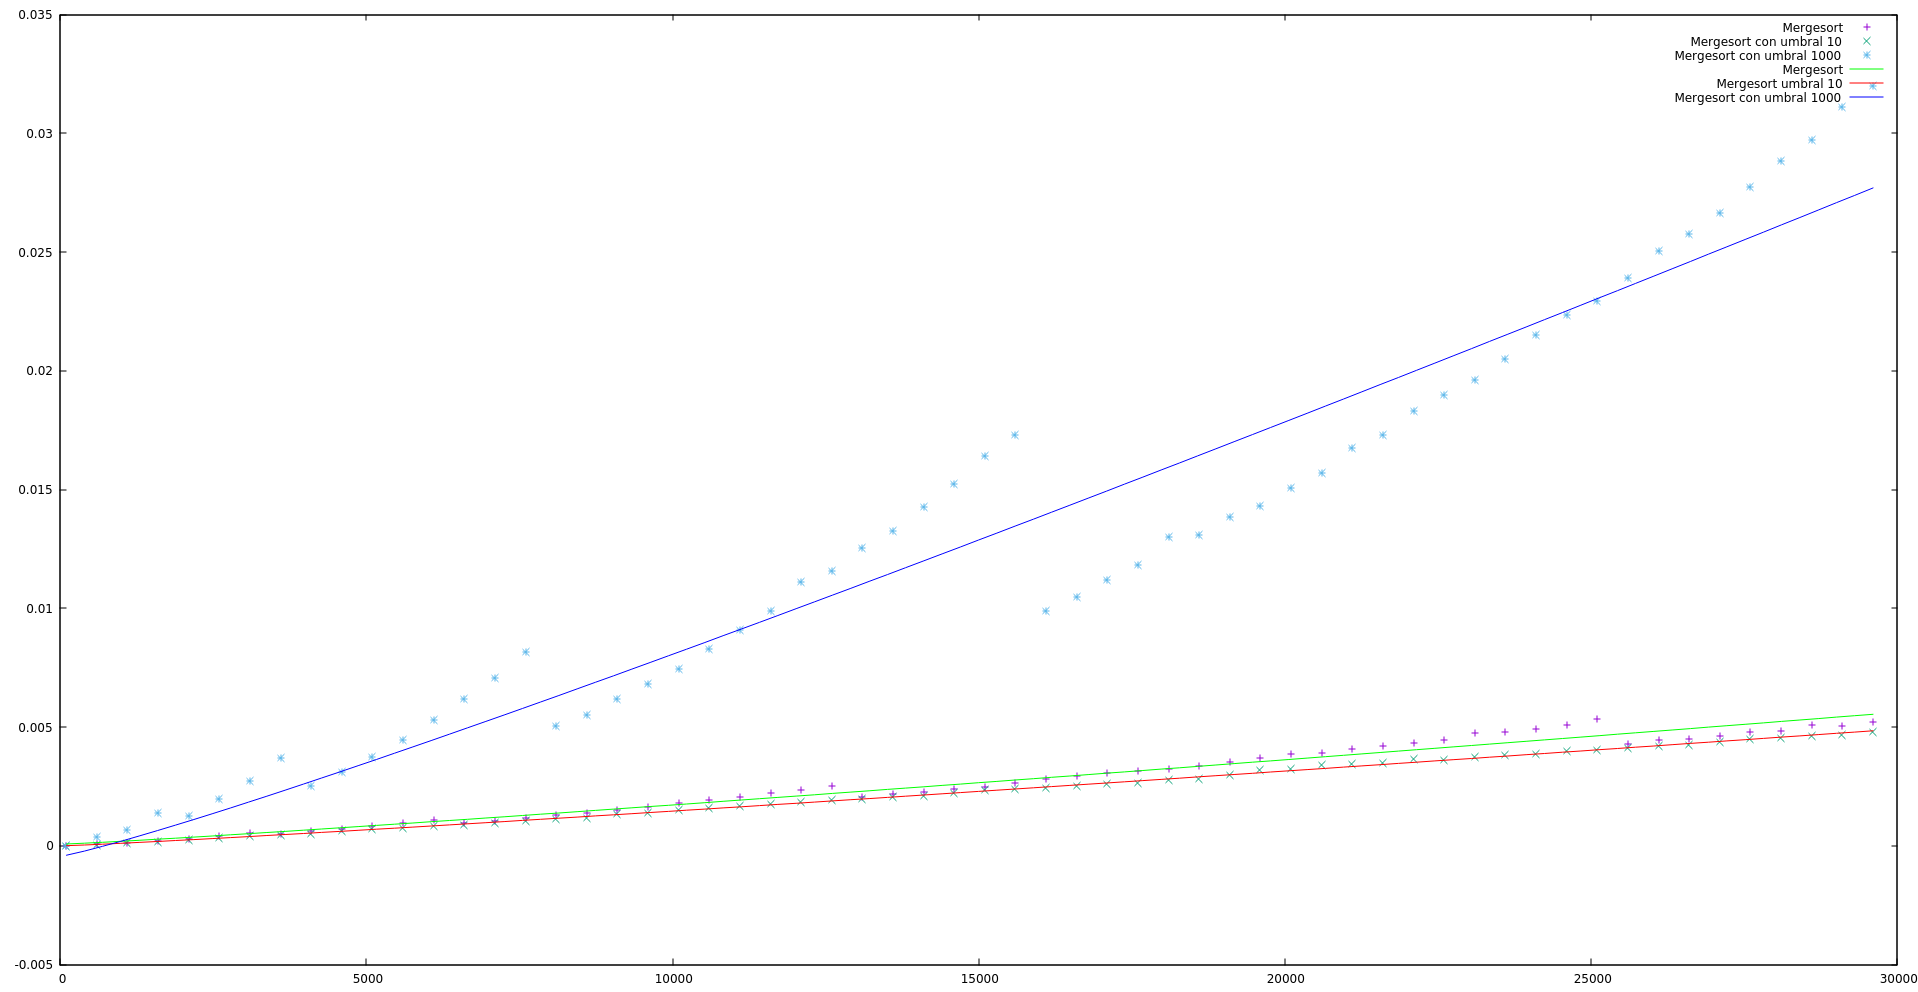
\includegraphics[width=0.9\textwidth]{ejer8/comparacion.png}
  \end{figure}
  